\hspace{0.5cm} In this paper, we employ a set of Spanish business news articles from Dow Jones Newswires for the period from 24/06/2020 to 30/09/2021. In total, we have 2,613 articles. The number of articles we work with and the time period over which they are spanned is a consequence of both data limitations and our filtering process. In particular, we want to focus the analysis on news articles pertaining to firms publicly traded in the IBEX-35. 



This paper employs a databse of Spanish business news articles sourced from DowJones and spanning from the 24 of Junes 2020 to the 30 of September 2021, a specially volatile period due to the Covid-19. The choice of dataspan is not casual, there are two reasons for this. 
We want to test a novel methodology in a reduced dataset, however, to gauge the extrapolative power of this methodology, the data sample should come from an unstable or volatile period, that's why we chose the covid-19 era. The articles are of high quality: they have been specifically filtered to mention IBEX-35 firms. The reason for this is that these are the 35 biggest companies in Spain by market capitalization, and hence, usually they are the most liquid and traded Spanish stocks, and also, the ones with the most consistent media coverage.

The use of DowJones Newswires as our news provider is not coincidental either. These news provider has the custom of writing the stock market ticker of the firms that are affected by the article between parenthesis, which eases a lot the process of extracting named entities from the news (also known as Named Entity Recognition). The type of ticker that is employed by DowJones is the one employed by YahooFinance to identify stocks, allowing for a seamless integration between our NER algorithm and the posterior trading with YahooFinance data.
In particular, by employing a pattern recognition algorithm (the \texttt{regex} library in Python), we can estract firm-specific mentions to Spanish IBEX-35 traded firms by simply looking for mentions to patterns "<WORD>.MC" for any <WORD>. For example, 


\mx 
%Our original database consisted of more than 8 thousand Spanish business articles. However, after
The filtering process consisted of keeping only the articles that explicitly mention the stock market tickers of IBEX-35 firms that are directly affected by the articles. This procedure delivers a high-quality database from which we can easily extract the set of firms affected by each article using pattern recognition (the \texttt{regex} functionality in Python). This is really useful as it allows us to match articles to firms without the need to manually read them, or to depend on expensive metadata from payable news portals.

\mx 
However, in the second part of the paper, we will do precisely that. We will feed our articles to a Large Language Model (LLM) and ask it to manually parse each article according to a predefined schema. Among other things, the LLM is asked to extract the firms that it believes are directly affected by the shocks described in each article. Thanks to the high quality of our filtered dataset, the correlation of the firms extracted by the LLM with those extracted by the pattern recognition algorithm is very high.

\mx 
For the analysis carried out in later sections, we divide the data into 3 splits: \textit{Train}, \textit{Validation}, and \textit{Test}. Each data split has a different functionality, which will become clear as we progress through the paper. In \cref{tab:Articles_Summary_Statistics} we provide the summary statistics of each data split. 


%In this study, we utilize the Factiva database, a comprehensive repository of global news and information sourced from thousands of newspapers, newswires, and publications. Factiva aggregates content from over 32,000 sources in 28 languages, offering a broad spectrum of economic news coverage. Access to the Factiva database was obtained through the Bank of Spain.
%
%\mx 
%Initially, our dataset comprised approximately 450,000 articles extracted from Spanish economic newspapers archived within the Factiva database; namely, the sources include \qquote{Cinco D�as}, \qquote{Expansi�n}, \qquote{El Economista}, \qquote{Reuters}, and \qquote{Dow Jones}. To focus our analysis on news pertaining to companies listed on the Ibex-35, a variable was employed to identify and extract articles featuring these entities. This filtering process yielded a subset of 8,108 articles relevant to our study. The sampled articles predominantly originated from \qquote{Dow Jones}, indicating a presumed level of reliability and credibility associated with the source. 

%----------------------------------------------------
\inserthere{tab:Articles_Summary_Statistics}

\begin{table}[H]
\centering
\caption{Summary Statistics of Articles by Data Split}
\label{tab:Articles_Summary_Statistics}
%\begin{tabular}{|l||c|c|c|c|}
\begin{tabular}{lcccc}
\hline \Xhline{2\arrayrulewidth}
%\rowcolor{gray!10}
\textbf{Data Split} & \textbf{Time Period} & \textbf{\# Articles} & \textbf{\# Words} & \textbf{Vocabulary Size} \\
\hline \Xhline{2\arrayrulewidth}
Train & 24/06/2020 $-$ 12/02/2021 & 1254 & 327413 & 26762 \\
Validation & 12/02/2021 $-$ 21/06/2021 & 836 & 232912 & 22265 \\
Test & 21/06/2021 $-$ 30/09/2021 & 523 & 140495 & 16474 \\ \hline \Xhline{\arrayrulewidth}
All & 24/06/2020 $-$ 30/09/2021 & 2613 & 700820 & 42603 \\ \hline \Xhline{2\arrayrulewidth}
\end{tabular}
\mx 
\subcaption*{\textit{Note: Summary statistics by data splits and for the whole sample. We provide the period spanned by each data split, the number of articles, the number of words, and the vocabulary size. Articles have been preprocessed following standard NLP practices.}}
\end{table}

%----------------------------------------------------


The most common words in the whole dataset are represented by means of a WordCloud, as shown in \cref{fig:WordCloud}. 

%The most common words across the whole sample (and the amount of times they are repeated) are: 
%\qquote{euro} (21,609), \qquote{millones} (14,370), \qquote{compa��a} (7,075), \qquote{a�o} (6,361), \qquote{nivel} (6,046), \qquote{banco} (5,754), \qquote{precios} (5,453), \qquote{resistencia} (4,545) and \qquote{plazo} (4,365). This is usually better represented in a Word Cloud (see \Cref{fig:word_cloud}). This Word Cloud was generated over a processed version of the articles. Namely, we collapsed all the news articles into a single document and applied the usuall processing steps (lowercase, tokenize, remove punctuation, stopwords and symbols, lemmatize and remove punctuation again). The vocabulary of the corpus initially consists of 33,579 different words, but removing words that appear too infrequently (only 1 time across all the sample) reduces the vocabulary to 21,564 words.

%----------------------------------------------------
\inserthere{fig:WordCloud}
\begin{figure}[H]
  \centering
  \caption{Word Cloud of the whole dataset}
  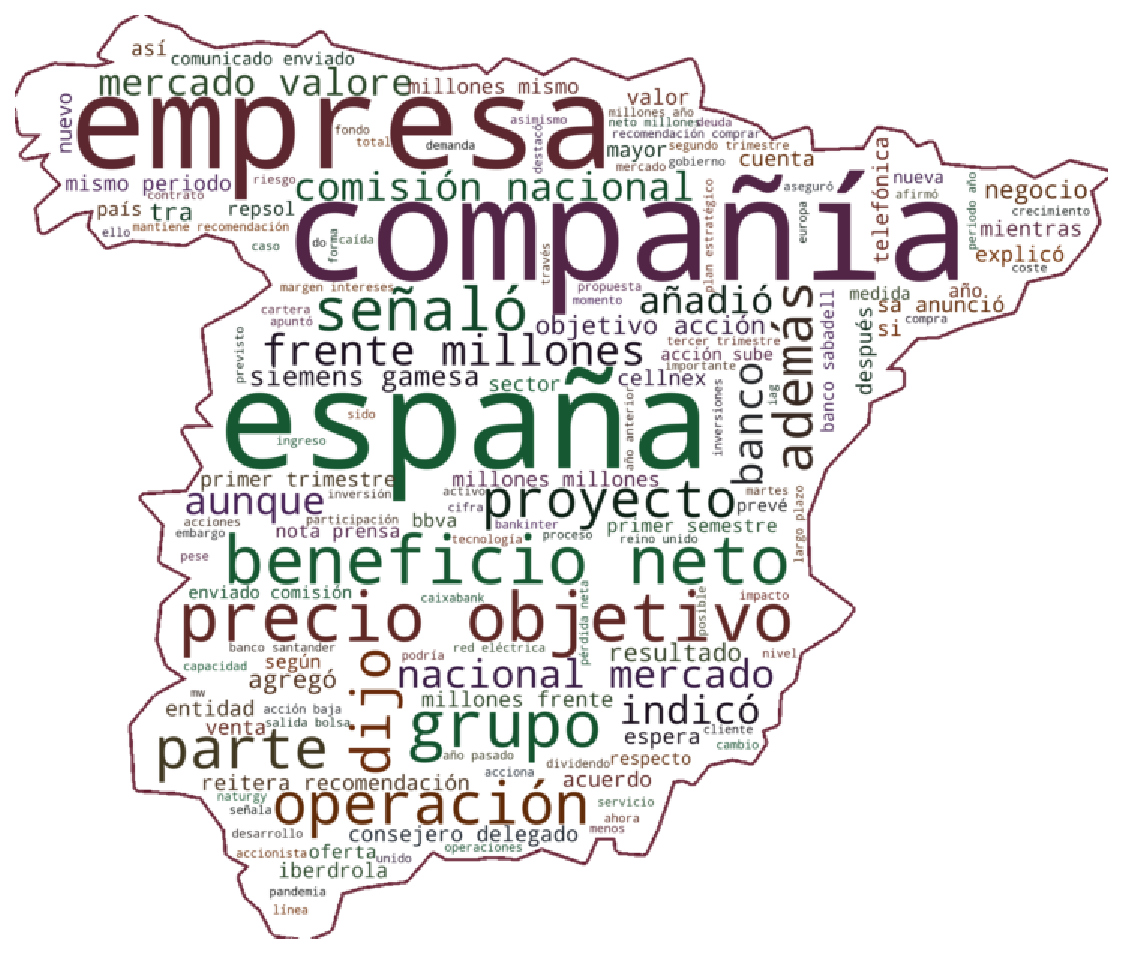
\includegraphics[scale=0.496]{/Users/jesusvillotamiranda/Library/CloudStorage/OneDrive-UniversidaddeLaRioja/CEMFI/__MSc__/__Second_year__/6th_Term/MasterThesis/__Output/EDA_WordCloud.pdf}
  \label{fig:WordCloud}
\end{figure}

%----------------------------------------------------


The distribution of the number of articles published per day is provided in \cref{fig:hist_1}, from where we see that the most common frequency of publication is between 5 and 10 articles per day, although there are days with unusually high publications. On the other hand, \cref{fig:hist_2} shows the distribution of number of words per article. Most of the mass is concentrated between 70 and 280 words per article, indicating relatively short articles that convey information straight to the point. However, we also observe some lengthy articles with over 500 words.  


%----------------------------------------------------
\inserthere{fig:histograms}
\begin{figure}[H]
  \caption{Histogram of \# News Articles per Day \& \# Words per Article}
  \centering
  \begin{subfigure}[b]{0.46\textwidth}
    \centering
    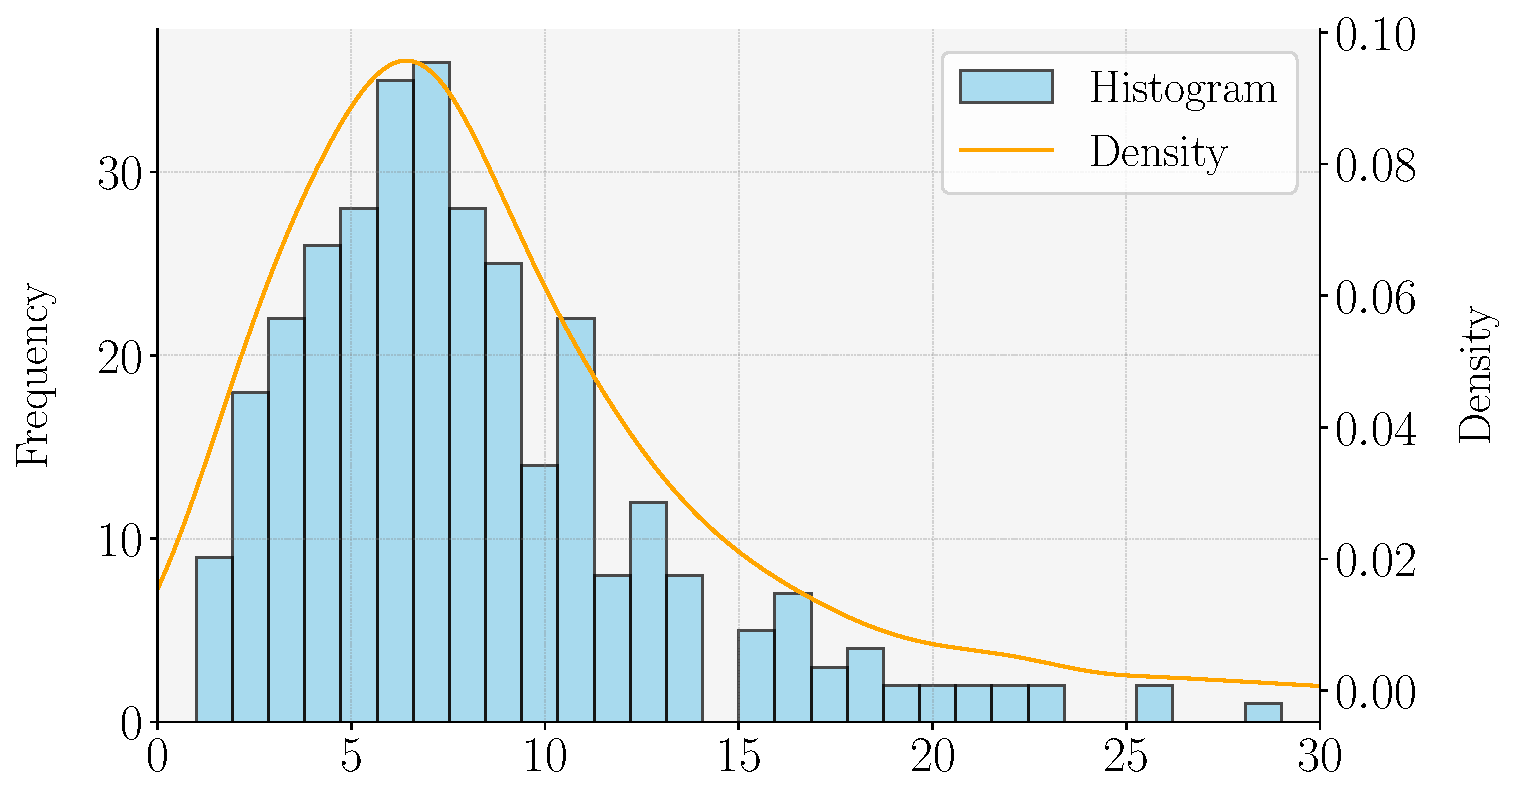
\includegraphics[width=\textwidth]{/Users/jesusvillotamiranda/Library/CloudStorage/OneDrive-UniversidaddeLaRioja/CEMFI/__MSc__/__Second_year__/6th_Term/MasterThesis/__Output/EDA_Histogram_of_Number_of_News_Articles_per_day.pdf}
    \caption{Number of News Articles per Day}
    \label{fig:hist_1}
  \end{subfigure}
  \hspace{0.05\textwidth} % Add horizontal space between the subfigures
  \begin{subfigure}[b]{0.46\textwidth}
    \centering
    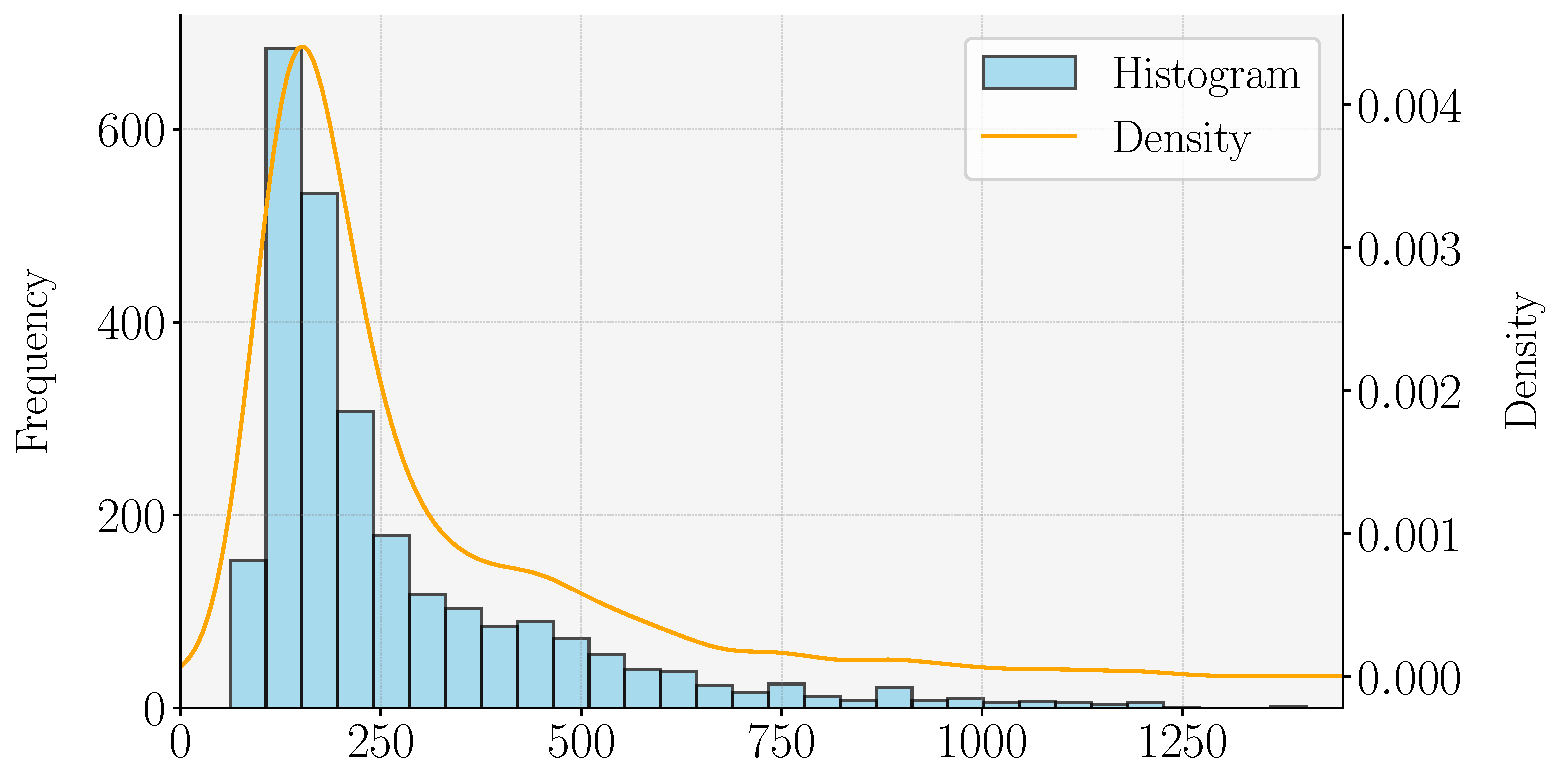
\includegraphics[width=\textwidth]{/Users/jesusvillotamiranda/Library/CloudStorage/OneDrive-UniversidaddeLaRioja/CEMFI/__MSc__/__Second_year__/6th_Term/MasterThesis/__Output/EDA_Number_of_Words_per_Article.pdf}
    \caption{Number of Words per Article}
    \label{fig:hist_2}
  \end{subfigure}
  \label{fig:histograms}
\end{figure}
%----------------------------------------------------


The time series of articles published per day throughout the sample timeline can be seen in \Cref{fig:ts_articles}. The series is quite spiky, jumping from low frequencies of publication (less than 5 articles in a day) to sudden spikes of more than 20 articles in a day. The moving average smoothes the series and confirms the previous observation that, on average, the number of articles published per day revolves between 5 and 10.

%----------------------------------------------------
\inserthere{fig:ts_articles}
\begin{figure}[H]
  \centering
  \caption{Time Series of Number of Articles per Day \& Moving Average (30 periods)}
  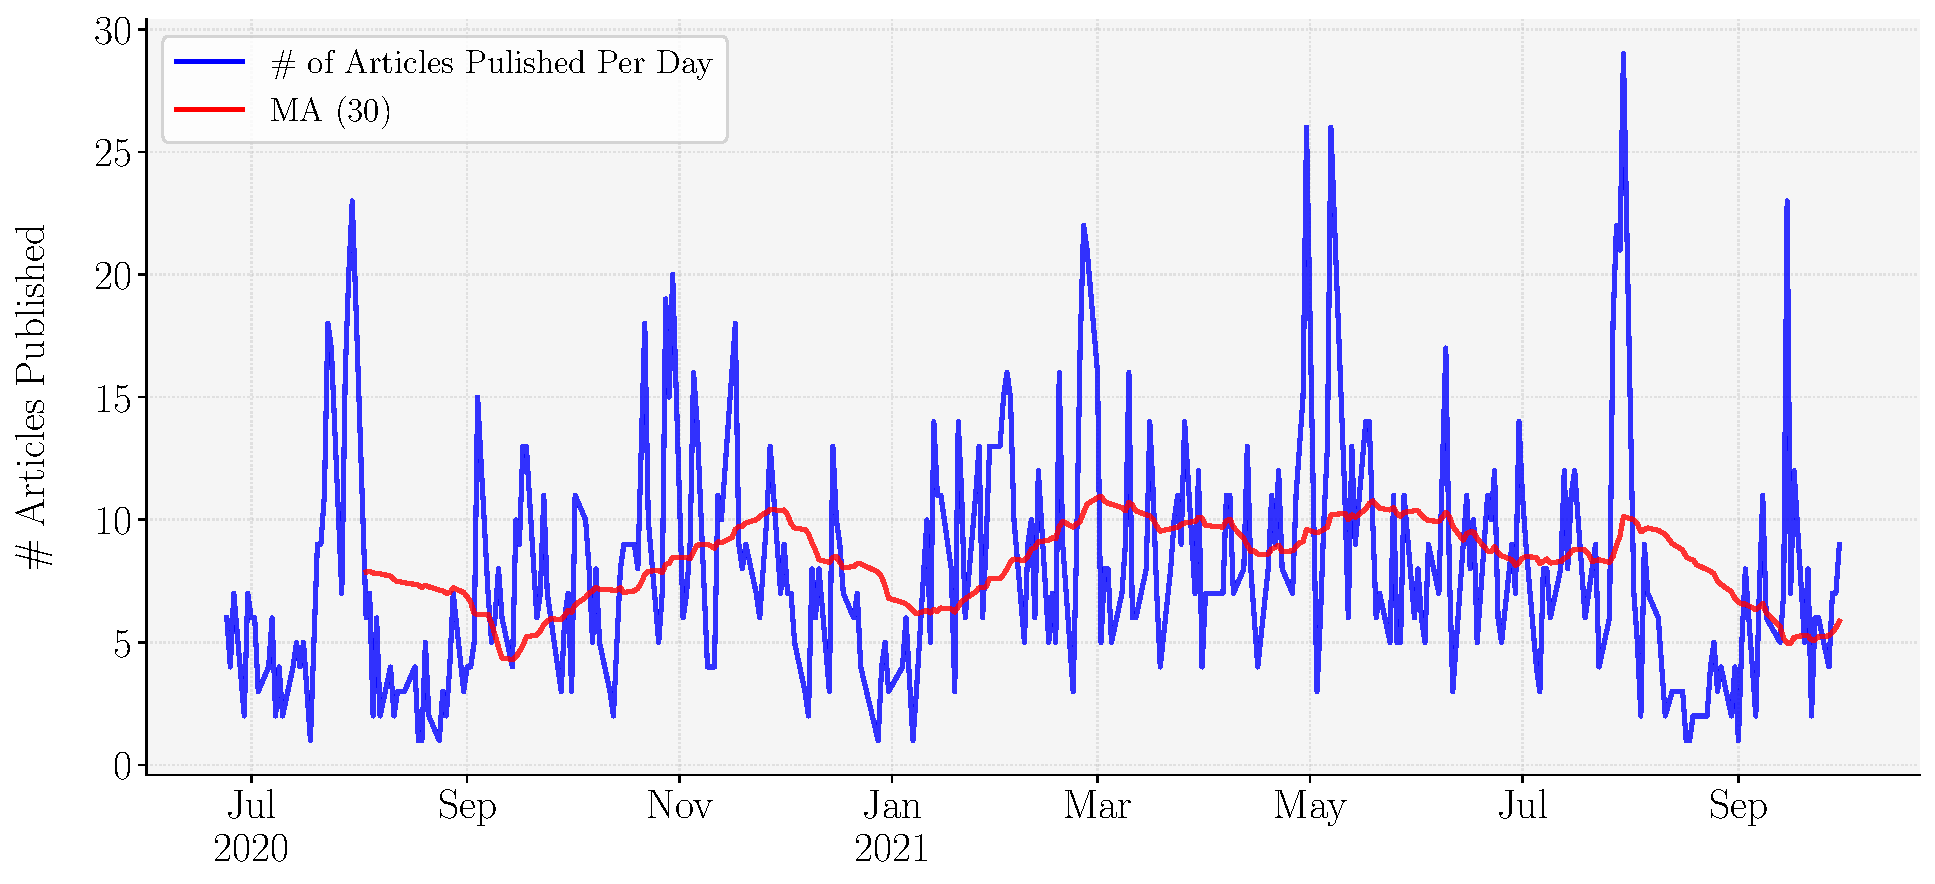
\includegraphics[scale=0.445]{/Users/jesusvillotamiranda/Library/CloudStorage/OneDrive-UniversidaddeLaRioja/CEMFI/__MSc__/__Second_year__/6th_Term/MasterThesis/__Output/EDA_Time_Series_of_Articles.pdf}
  \label{fig:ts_articles}
\end{figure}
%----------------------------------------------------

